\documentclass{article}
\usepackage{graphicx,listings,lmodern,luatextra,dtklogos}
\newcommand\pkgversion{see Makefile}

\newcommand*\pgsmall{\fontsize{8.5}{8.7}\selectfont\ttfamily}
\lstset{basicstyle=\pgsmall,
  basewidth=0.55em,
  columns=fullflexible,
  breakautoindent=true,
  breaklines=true,
  prebreak=,
  postbreak=\mbox{$\hookrightarrow$},
}

\begin{document}
\title{The lua-visual-debug package (V\pkgversion)}
\author{Patrick Gundlach}
% \address{patrick@gundla.ch}
\maketitle

\tableofcontents
\section{About}

This package aids debugging your \TeX\ and \LaTeX\ document by drawing rectangles around boxes and rules where glue is inserted. Other items are marked as well: kerns, hyphenation points and penalties.

\section{How to use}

When you load the package \texttt{lua-visual-debug} in your \LuaLaTeX\ document (or use \verb|\input lua-visual-debug.sty| in plain \TeX), \LuaTeX\ will highlight boxes, penalties, glues and kerns in the PDF. This package requires you to process the document with \LuaTeX\ (plain and \LaTeX formats).

\section{A \LaTeX\ example}
\lstinputlisting[language=tex]{sample.tex}

\noindent yields \vspace{5mm}

\noindent \includegraphics[width=\textwidth]{sample-crop.pdf}

\section{A plain \TeX\ example}

\lstinputlisting[language=tex]{sample-plain.tex}

\noindent yields \vspace{5mm}

\noindent \includegraphics{sample-plain-crop.pdf}

\section{How to interpret the markers} % (fold)
\label{sec:how_to_interpret_the_markers}

\noindent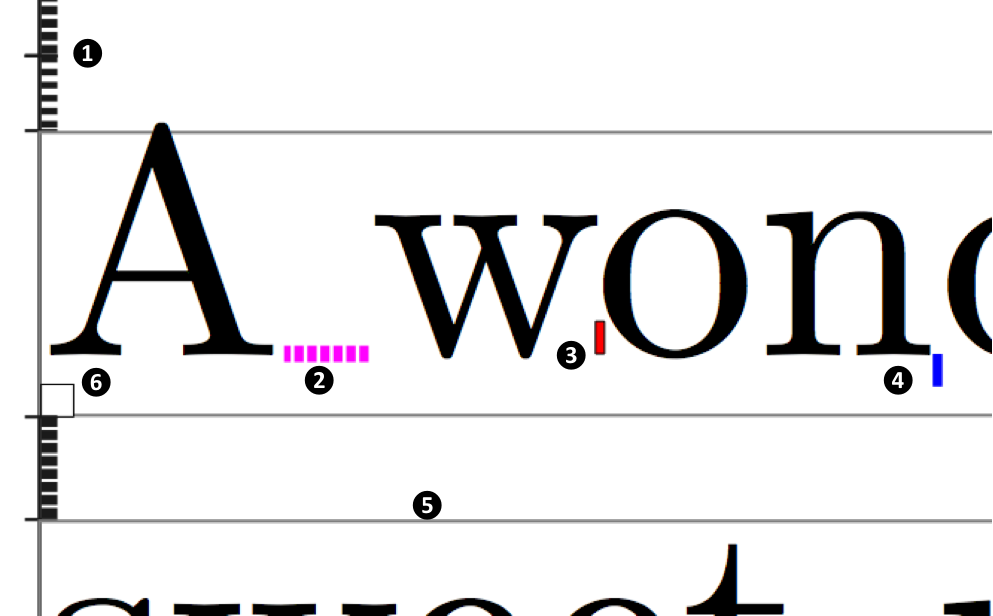
\includegraphics[width=.9\textwidth]{lvdebugdetail1-num}
\begin{enumerate}
	\item A vertical glue. Beginning and end are marked with a small tick. At the mark 1, two vertical glues are connected.
\item A horizontal glue.
\item A negative kern. Positive kerns are yellow.
\item A possible hyphenation point.
\item Horizontal and vertical boxes are drawn with a border.
\item Penalties are marked with a square. A penalty of 10,000 is marked with a blank square, a penalty less than 10,000 is filled with a gray square (that will improve in the future, currently it is grayness of penalty / 10000).
\end{enumerate}

A strut box (zero width box) is marked with a red rule:

\noindent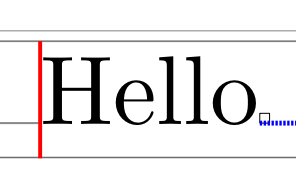
\includegraphics[scale=0.8]{strut}

% section how_to_interpret_the_ (end)


\section{Copying}

Copyright 2012 Patrick Gundlach (patrick@gundla.ch), licensed under the MIT license. See the Lua file for details.


\end{document}
